\begin{appendices}

\section{\acf{he} Multiplication}
\label{app:he-multiplication}

In this section, we proof how the multiplication is achieved homomorphically between two encrypted vectors $[[x'_1]], [[x'_2]]$, as described in \cite{liu2016efficient2}.
It is worth mentioning that $[[x'_i]] = [[x_i]]^{r_{x_i}} = [[x_i . r_{x_i}]]$.
This step is performed for masking the value $x_i$ by adding a random value $r_{x_i}$ to it.
The formal definition of this function is $\ac{he}.Mul([[x'_1]], [[x'_2]]) \rightarrow [[x_{mul}]]$.
\Cref{fig:he-mul-explain} shows the operations for performing the multiplication operation between two parties $S_1, S_2$, where they hold the homomorphic secret key $sk_1, sk_2$, respectively.

\begin{figure*}[thb]
\centering
  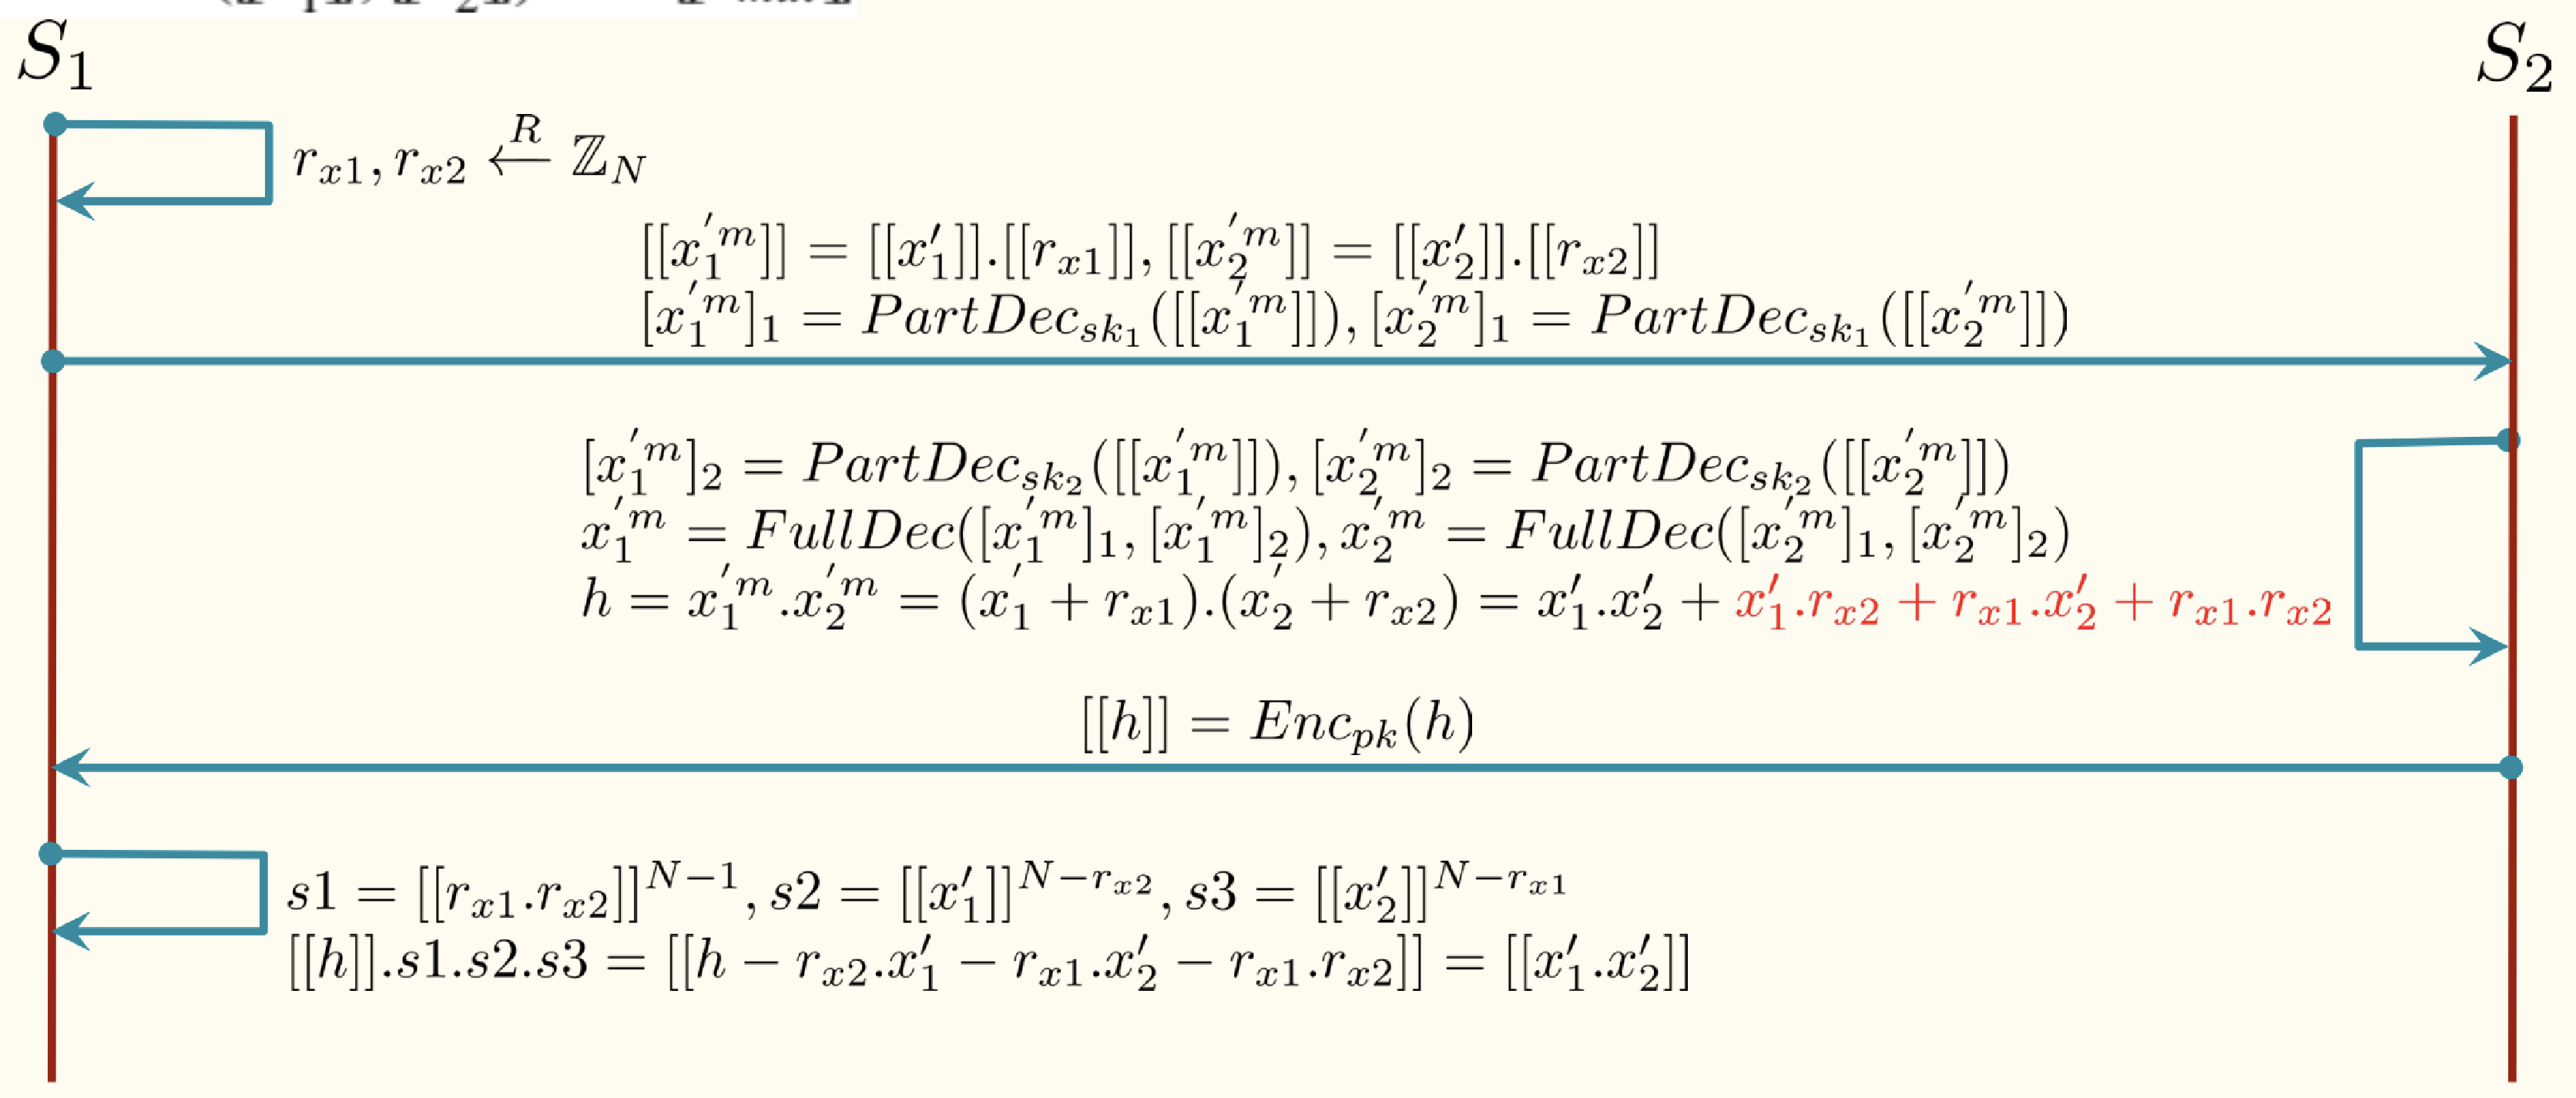
\includegraphics[width=0.8\linewidth]{resources/HE-mul-explain.pdf}
  \caption{HE multiplication explanation}
  \label{fig:he-mul-explain}
  %\vspace{-5mm}
\end{figure*}
    
\section{Normalization Judgement}
\label{app:normalization-judgement}

$SecJudge$ algorithm depicted in \Cref{fig:sec-judge-impl}, takes the encrypted gradient $[[g_i]]$ from a user and returns $Accept$ if the encrypted gradient is normalized or $Reject$ otherwise.
It is worth mentioning that the gradient consists of a list of $m$ values associated with the training model weights, as shown in the first line.
In equation 14, $S_1$ adds a random value to mask the gradient value $x'_k$.
This masking is important because later, as the algorithm progresses, $S_1$ will share this value with $S_2$.
That is why it masks the value before sharing it with $S_2$.
As mentioned previously, the multiplication of two homomorphically encrypted vectors will result in the encrypted addition of the plaintext values inside those ciphertexts.
In addition, $S_1$ partially decrypts the ciphertext after masking $[[\bar{x}_k]]$ using its secret key $sk_1$ to produce $[\bar{x}]_1$, and shares it with $[[x']]$ with $S_2$.
On the other hand, $S_2$ performs a partial decryption on the value $[[\bar{x}]]$ using its secret key $sk_2$ to get the value $[\bar{x}]_2$.
Using both values $[\bar{x}]_1$, from $S_1$, and $[\bar{x}]_2$, $S_2$ performs a full decryption to get the masked value $\bar{x}$.
Then, $S_2$ calculates $\bar{x}_k^2$ and shares their summation after encrypting it, resulting in: $[[\sum \bar{x}_k^2]]$, with $S_1$.
Moreover, $S_1$ unmasks the value to get the encrypted value that represents the unmasked sum of the gradients $[[sum]]$ in equation 15.
Then it decrypts it with the help of $S_2$ to get the value $sum$.
Finally, it is easy to know if this value sums to one, then accept or reject otherwise.

\begin{figure}[htb]
\centering
  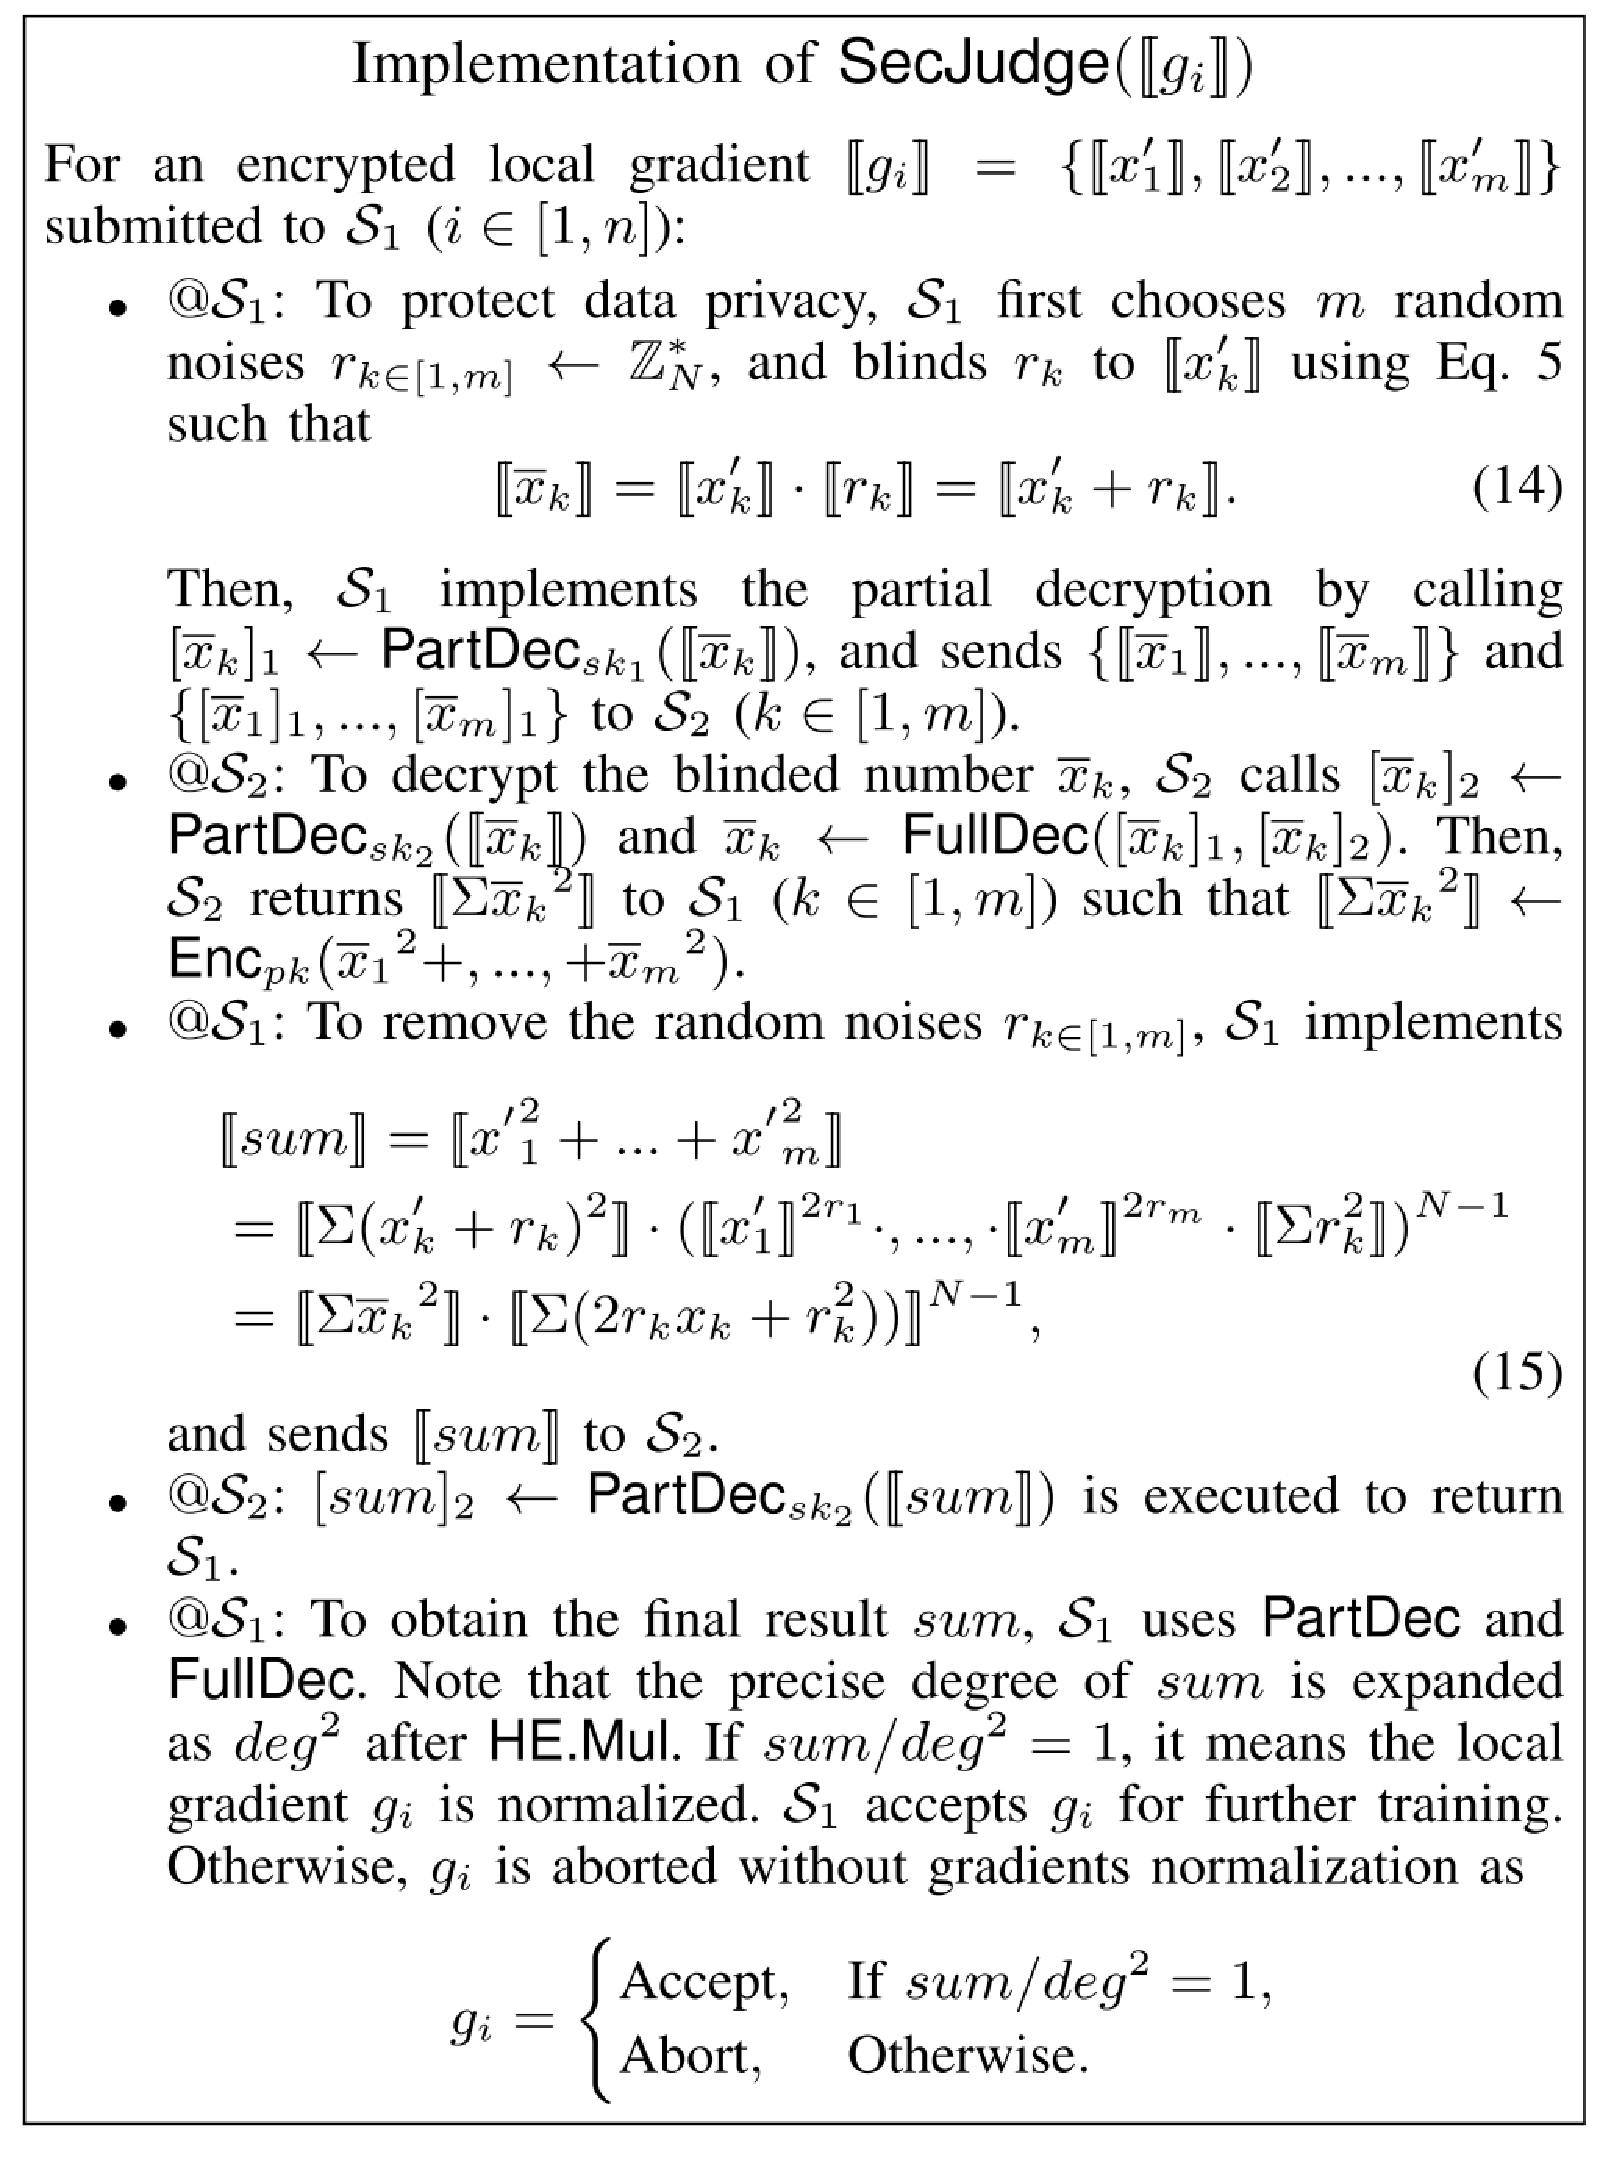
\includegraphics[width=0.8\linewidth]{resources/sec-judge-impl.pdf}
  \caption{Normalization judgement implementation details}
  \label{fig:sec-judge-impl}
  %\vspace{-5mm}
\end{figure}

\section{Cosine Similarity}
\label{app:cos-similarity}

\Cref{fig:sec-cos-impl} depicts the details of the cosine similarity algorithm that decides if two encrypted vectors $[[g_a]], [[g_b]]$ are similar or not.
The process is very similar to what has been explained in \Cref{app:normalization-judgement}.
First, $S_1$ masks both vectors to create the values $[[\bar{g}_a]], [[\bar{g}_b]]$.
Then it shares them with the following values with $S_2$: $[[\bar{g}_a]], [[\bar{g}_b]], [\bar{g}_a]_1, [\bar{g}_b]_2$.
Then, $S_2$ performs full decryption to get the values $\bar{g}_a, \bar{g}_b$.
Moreover, it multiplies both vectors to calculate the cosine similarity $\bar{cos}_{ab}$.
After that, it encrypts it to produce $[[\bar{cos}_{ab}]]$ and shares it with $S_1$.
With the help of $S_2$, $S_1$ decrypts the cosine similarity value after removing the masking from it, $cos_{ab}$.

\begin{figure}[thb]
\centering
  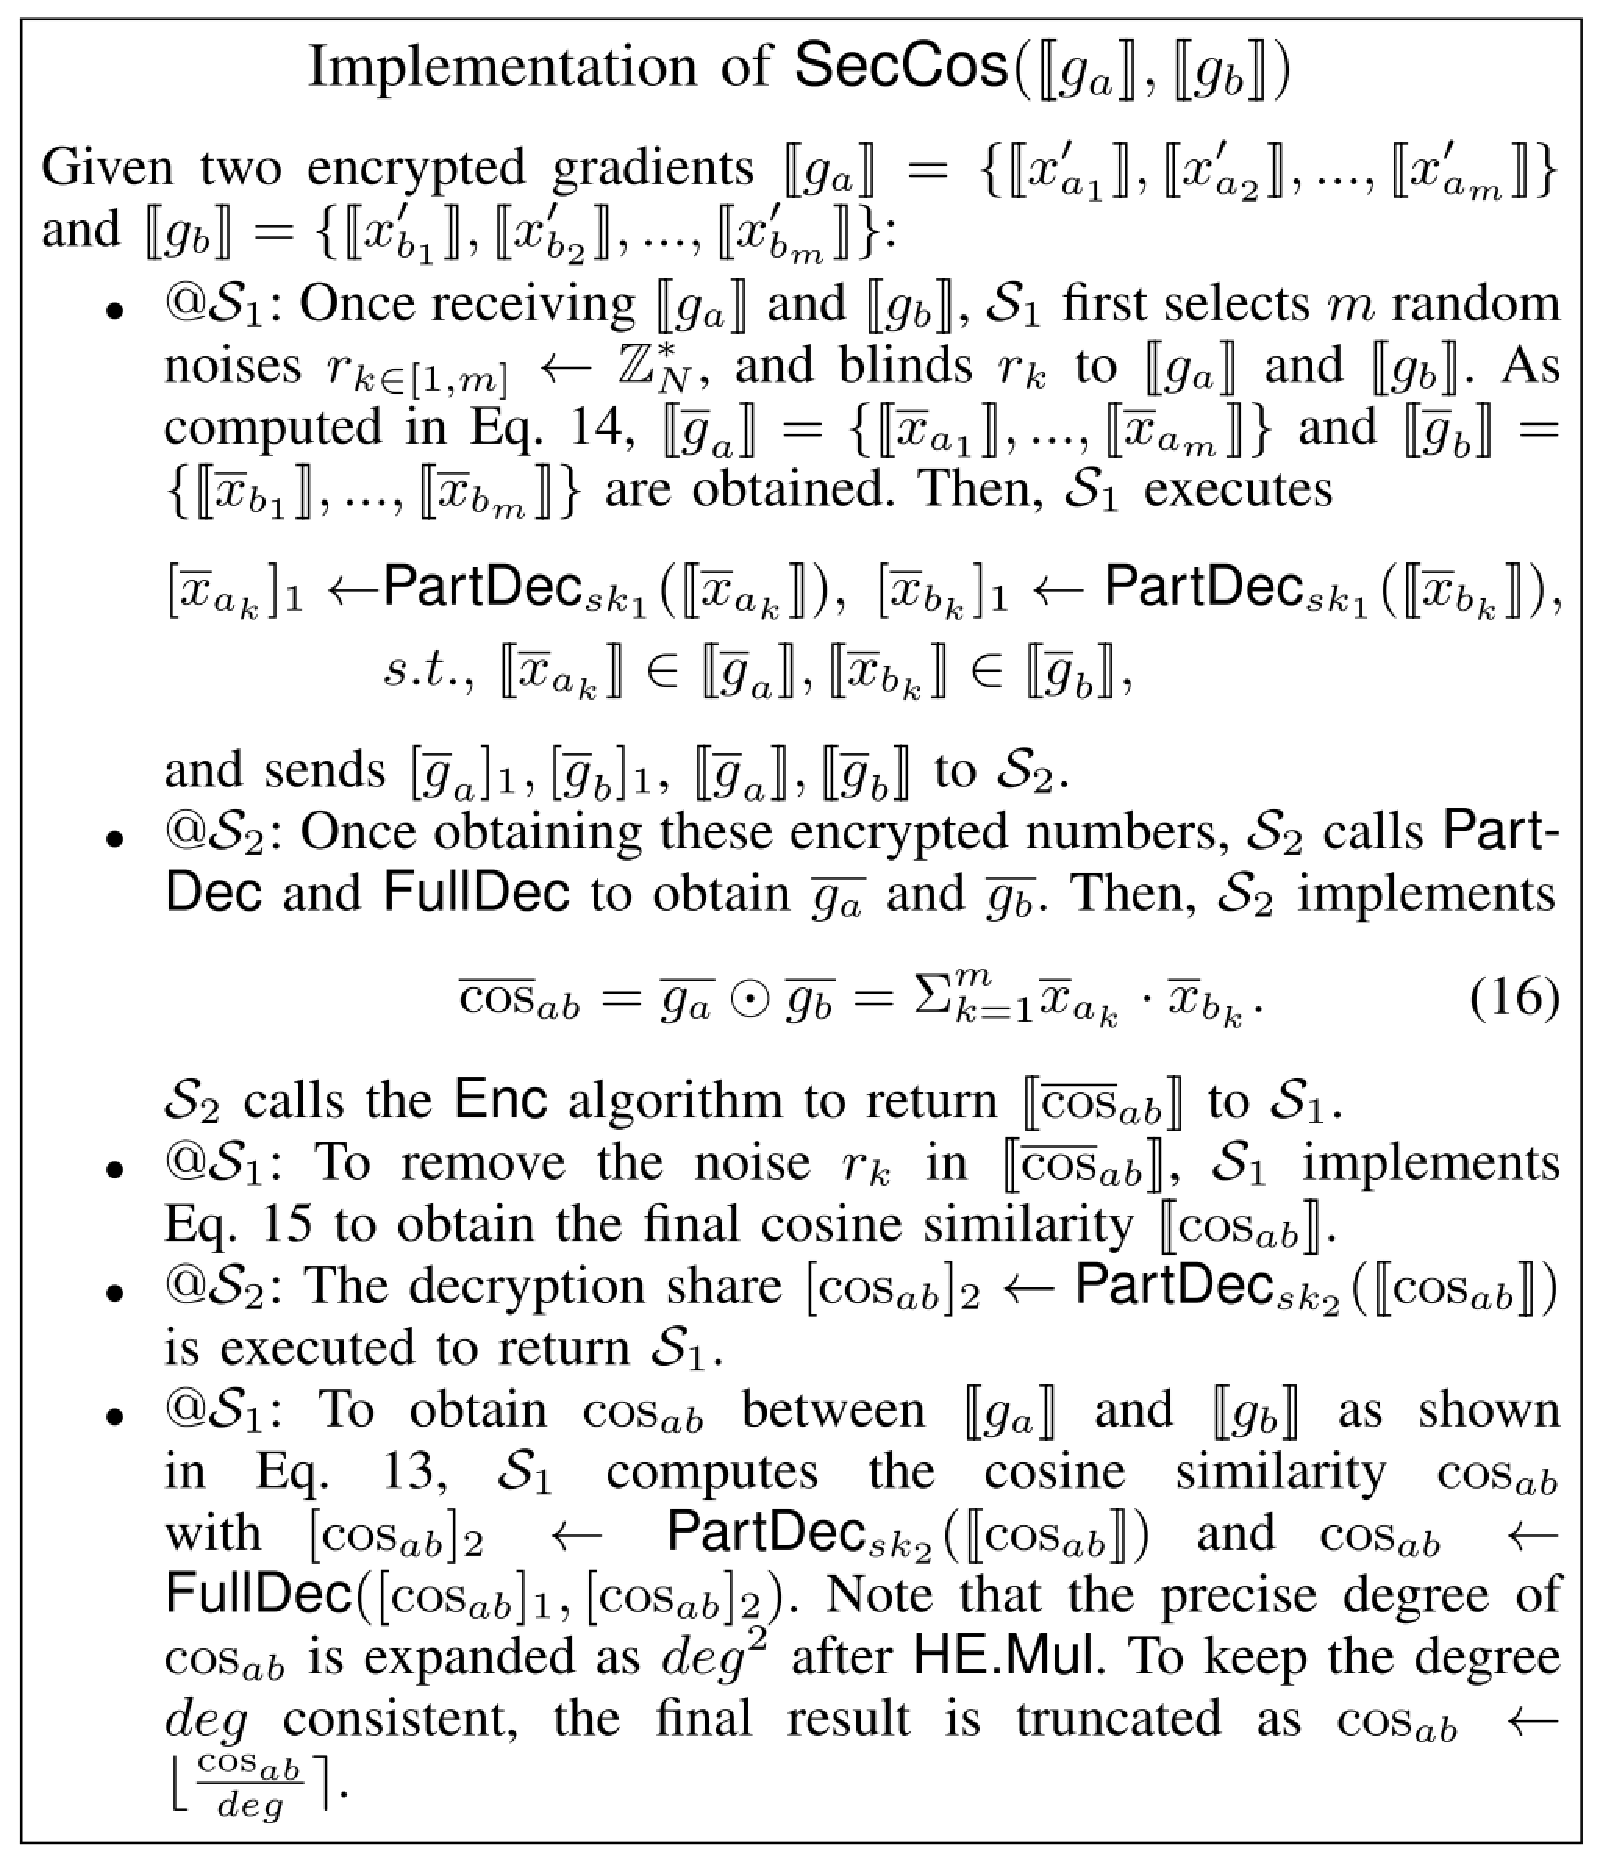
\includegraphics[width=0.8\linewidth]{resources/sec-cos-impl.pdf}
  \caption{Cosine similarity implementation details}
  \label{fig:sec-cos-impl}
  %\vspace{-5mm}
\end{figure}

\end{appendices}
